\chapter{Аналитический раздел}
\section{Формализация задачи}

% TODO: пользователь или оператор
% Описать кто такой эксперт, кто такой пользователь и тд (привязываемся к конкретике данной задачи)
Задача сопровождения оператора при выполнении инструкции состоит в поддержке и руководстве действиями пользователя для достижения нужного результата, обеспечения выполнения задач~\cite{sadovnik}.
Она включает пошаговые подсказки, отслеживание прогресса, помощь в случае ошибок и адаптацию действий под новые требования, обусловленные развитием событий по ходу решения оператором задачи.

На рисунке~\ref{A0} представлена формализация задачи  поддержки пользователя при выполнении инструкции в виде IDEF0 диаграммы.

\begin{figure}[H]
	\centering
	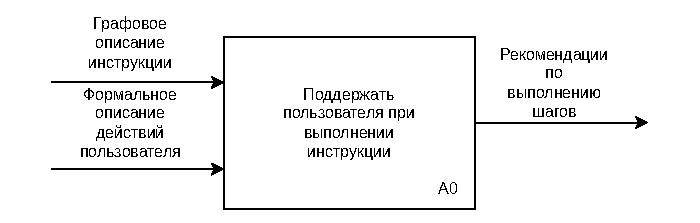
\includegraphics[width=0.9\linewidth]{inc/img/idef05.pdf}
	\caption{Формализация задачи поддержки пользователя при выполнении инструкции}
	\label{A0}
\end{figure}

\clearpage

\section{Системы поддержки принятия решений}
\subsection{Основы теории принятия решений}
Системы поддержки принятия решений являются результатом развития теории принятия решений и последующим повышением сложности используемых методов.
Следовательно, для полноценного анализа предметной области необходимо рассмотреть основные понятия предметной области теории принятия решений.

\textbf{Теория принятия решений} --- это совокупность методов и моделей, предназначенных для обоснования решений, принимаемых на этапах анализа, разработки и эксплуатации сложных систем различной природы: информационных, технических, производственны, организационных и экономических~\cite{chernomor}.
\textbf{Принятием решения} называется выбор одной из нескольких альтернатив.
В качестве отличительной особенности методов принятия решений можно выделить их ориентированность на решение задач, встречаемых в человеческой деятельности.
Применимость методов принятия решений зависит от рассматриваемой проблемы.
С точки зрения методов принятия решений все проблемы делятся на три класса~\cite{foundations}:
\begin{itemize} 
    \item \textbf{хорошо структурированные}, или количественно сформулированные --- проблемы, в которых зависимости полностью сформулированы;
    \item \textbf{неструктурированные}, или качественно выраженные --- проблемы, содержащие описание лишь части ресурсов, признаков и характеристик, отсутствует информация об их количественных зависимостях;
    \item \textbf{слабо структурированные}, или смешанные --- содержат как качественные элементы, так и неизвестные.
\end{itemize}

Методы теории принятия решений в основном ориентированы на решение структурированных задач, где возможно найти количественные зависимости между параметрами исследуемой системы и критериями эффективности~\cite{larichev}.

В процессе принятия решений можно выделить несколько ролей. 
\textbf{Субъект принятия решения}, то есть лицо, фактически осуществляющее выбор наилучшего варианта действий, называют лицом, принимающим решение (ЛПР). 
Лицо, ответственное за принятие решения, называют \textbf{владельцем проблемы}. 
ЛПР и владелец проблемы не обязаны совпадать. 
Также выделяют роли \textbf{руководителя} или \textbf{участника активной группы} --- группы лиц, оказывающих влияние на процесс принятия решений. 
Человек также может выступать в роли \textbf{эксперта}, то есть профессионала в некоторой области, и способен давать оценки и рекомендации.
Последней ролью является \textbf{консультант} по принятию решений. 
Его роль состоит в организации процесса организации решений.

Для сравнения нескольких вариантов при принятии решения каждое из них характеризуют различными показателями, которые указывают на предпочтительность варианта для ЛПР.
Такие параметры называют \textbf{критериями оценки}.

Задача принятия решений заключается в структурированном выборе наилучшей альтернативы для достижения одной или нескольких целей в условиях неопределённости и при наличии ограниченных ресурсов~\cite{larichev}.
\textbf{Альтернативой} называется вариант действий.
Наилучшая альтернатива определяется в результате сравнения по критериям оценки.
Для постановки задачи принятия решений необходимо хотя бы две альтернативы.

В задаче принятия решений выделяют несколько этапов.
\begin{enumerate} 
    \item Сбор всех доступных данных на момент принятия решения.
    \item Определение возможных альтернатив.
    \item Сравнение альтернатив и выбор наилучшего варианта решения.
\end{enumerate}


Если при сравнении двух альтернатив одна из них превосходит другую по всем критериям оценки, то эта альтернатива называется \textbf{доминирующей} по отношению к другой.
Так как критерии оценки характеризуют предпочтительность варианта для ЛПР, доминирующие альтернативы считаются более оптимальными по сравнению с теми, по отношению к которыми они доминируют.
Таким образом, если в результате сравнения окажется, что одна из альтернатив является доминирующей по отношению ко всем остальными, она будет считаться оптимальной и задача будет решена.

Если в результате попарных сравнений всех решений остаются несколько альтернатив, доминирующих над всеми остальными, помимо друг друга, выбор оптимального решения становится неочевидным~\cite{chernomor}.
В этой ситуации говорится, что оставшиеся альтернативы принадлежат \textbf{множеству Эджворта--Парето}.
Выбор оптимального решения из множества Эджворта--Парето является одной из основных задач принятия решений.

Выбор оптимальной альтернативы из множества на практике часто оказывается трудоёмкой операцией.
Для упрощения поиска создаются \textbf{системы поддержки принятия решений} (СППР) --- компьютерные автоматизированные системы, целью которых является частичная автоматизация выбора наилучшего решения в сложных условиях для полного и объективного анализа предметной деятельности~\cite{starodubcev}.

Таким образом, СППР предназначена для решений двух основных задач~\cite{larichev}:
\begin{itemize} 
    \item \textbf{оптимизация} --- выбор оптимального решения из множества возможных;
    \item \textbf{ранжирование} --- упорядочивание возможных решений по предпочтительности.
\end{itemize}

СППР, использующие методы искусственного интеллекта, называются интеллектуальными.

\subsection{Структура систем поддержки принятия решений}
В СППР выделяют следующие основные компоненты~\cite{concepts}:
\begin{itemize} 
    \item компонент механизм логического вывода --- отвечает за хранение и извлечения данных;
    \item компонент работы с моделями --- отвечает за работу с аналитическими моделями;
    \item компонент пользовательского интерфейса --- позволяет пользователям взаимодействовать с системой;
    \item компонент базы знаний --- хранит правила и экспертные заключения, необходимые для предоставления рекомендаций.
\end{itemize}

На рисунке~\ref{A2} изображена концептуальная схема СППР.

\begin{figure}[H]
	\centering
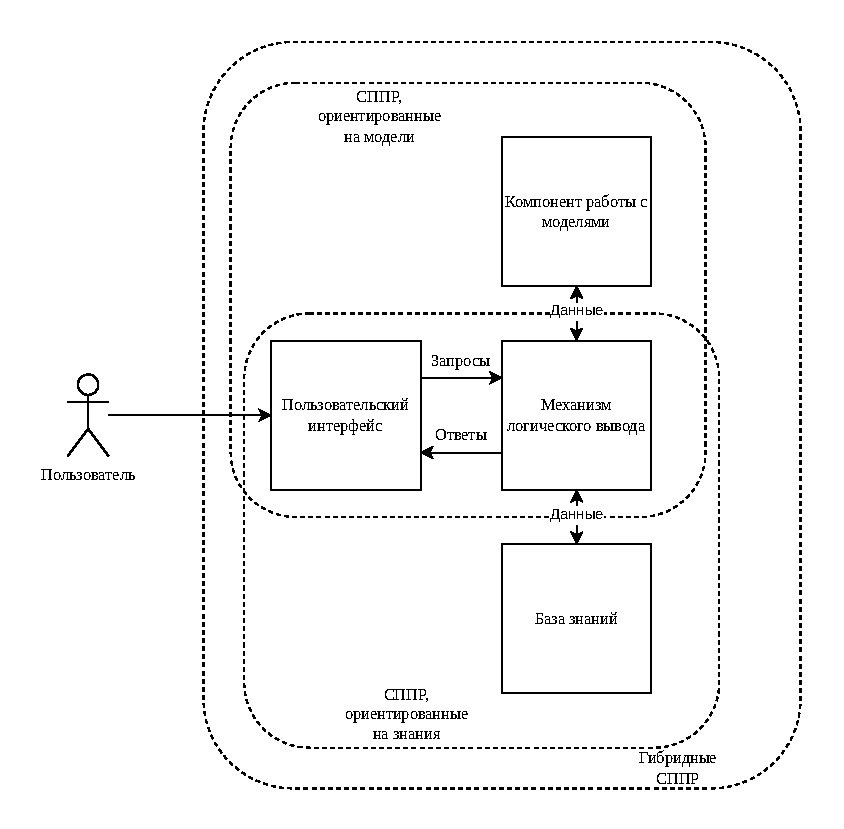
\includegraphics[width=0.6\linewidth]{inc/img/architecture.pdf}
	\caption{Концептуальная схема СППР}
	\label{A2}
\end{figure}


\subsection{Классификация систем поддержки принятия решений}
Существует множество способов классифицировать СППР, среди них выделяются следующие основные критерии~\cite{starodubcev}:
\begin{itemize} 
    \item по взаимодействию с пользователем;
    \item по способу поддержки.
\end{itemize}

По взаимодействию с пользователем выделяют следующие типы:
\begin{itemize} 
    \item \textbf{пассивные} --- не выдвигают решения, поддерживают ЛПР в процессе принятия решения;
    \item \textbf{активные} --- способны выдвигать собственные решения поставленной задачи;
    \item \textbf{кооперативные} --- разрабатывают собственные решения, корректируемые пользователем, итеративно достигая правильного решения. 
\end{itemize}

По способу поддержки выделяют следующие типы:
\begin{itemize} 
    \item ориентированные на данные --- работают с большим объёмом хорошо структурированных данных, предоставляя пользователю структурированные наборы фактов, полученные в результате анализа;
    \item ориентированные на документы --- используют в работе неструктурированные данные в различных электронных форматах, поддерживают пользователя, облегчая работу с большим объёмом документов;
    \item ориентированные на модели --- в своей работе используют финансовые, статистические и математические модели, позволяют менять входные параметры для тестирования и оптимизации результатов;
    \item ориентированные на знания --- используют в работе факты и правила для решения специализированных проблем, в основе лежит база знаний и набор правил, описанные экспертами;
    \item коммуникационные --- поддерживают совместную работу нескольких пользователей над общей задачей.
\end{itemize}

В данной работе выделяется особое внимание системам поддержки принятия решений, сопровождающих выполнение предписаний человеком.
СППР, ориентированные на данную задачу, относятся к ориентированным на знания, так как для каждого домена инструкций требуются индивидуальные размеченные экспертами рекомендации.

\subsection{Методы поддержки принятия решений}
Существует множество методов поддержки принятия решений~\cite{obzor}:
\begin{enumerate} 
    \item информационный поиск;
    \item интеллектуальный анализ данных;
    \item поиск знаний в базах данных;
    \item рассуждение на основе прецедентов;
    \item имитационное моделирование;
    \item эволюционные вычисления и генетические алгоритмы;
    \item нейронные сети;
\end{enumerate}

\textbf{Информационный поиск} --- процесс поиска неструктурированной документальной информации и наука об этом поиске.

Поиск информации представляет собой процесс выявления в некотором множестве тех из них, которые удовлетворяют заранее определённому условию поиска или содержат соответствующие запросу данные.

\textbf{Интеллектуальный анализ данных} --- процесс поиска закономерностей и взаимосвязей в больших массивах необработанных данных.
Занимается задачами классификации, моделирования и прогнозирования.

\textbf{Поиск знаний в базах данных} --- процесс поиска полезной информации в базах данных.
Эта информация может представлять из себя закономерности, правила, прогнозы.

\textbf{Рассуждение на основе прецедентов} --- подход поддержки принятия решений, основанный на использовании решений уже известных задач для новых задач. 

Основной целью рассуждения на основе прецедентов является поиск похожих случаев в базе данных, адаптация их решений к текущим условиям и сохранении нового опыта.

\textbf{Имитационное моделирование} --- метод, основанный на создании модели реальной системы и проведения экспериментов над ней с целью получения информации об этой системе.
Является частным случаем математического моделирования, используется при невозможности создания аналитической модели.

\textbf{Генетические алгоритмы} --- метод, основанный на эвристическом алгоритме поиска, используется для решения задач оптимизации путём последовательного подбора и комбинации искомых параметров с помощью действий, схожих с методами эволюции.

В основе генетических алгоритмов лежит оператор скрещивания, выполняющий создание новых решений путём комбинации оптимальных решений предыдущей итерации алгоритма.

\textbf{Нейронные сети} --- метод, в основе которого лежит построение математических моделей, схожих по организации и функционированию биологическим нейронным сетям.
\clearpage

\section{Графовый формат инструкций}
\label{graph_format}
Для организации сопровождения пользователя при выполнении инструкций необходимо преобразовать слабоструктурированный текст инструкции в подходящий единый формат, пригодный для обработки с помощью СППР.
Для достижения этой цели в данной работе будет рассматриваться специальный графовый формат.

Необходимость специального графового формата обусловлена недостаточностью широко используемых графовых форматов.

Любую инструкцию можно описать с помощью сущностей, действий, проводимыми над сущностями, и состояниями, между которыми сущности переходят в процессе выполнения.
Так как сразу несколько сущностей могут проходить через одни и те же состояния, они выделяются в отдельные объекты на графе --- состояния контекста.
Для представления всех трёх объектов на одном графе предлагается графовый формат, сочетающий идеи \textbf{сетей Петри}, позволяя представлять состояния и переходы между ними, и \textbf{семантической сети}, позволяя представлять сущности и их отношения к состояниям.

Таким образом, в узлах размещается состояние контекста и действия, приводящие к изменению состояний.
Состояния контекста ссылается на сущности, между которым установлены семантические связи, такие ссылки могут быть множественными и бывают двух видов: текущие объекты и текущие субъекты.

На рисунке~\ref{A1} приведён пример графа в описанном формате.

\begin{figure}[H]
	\centering
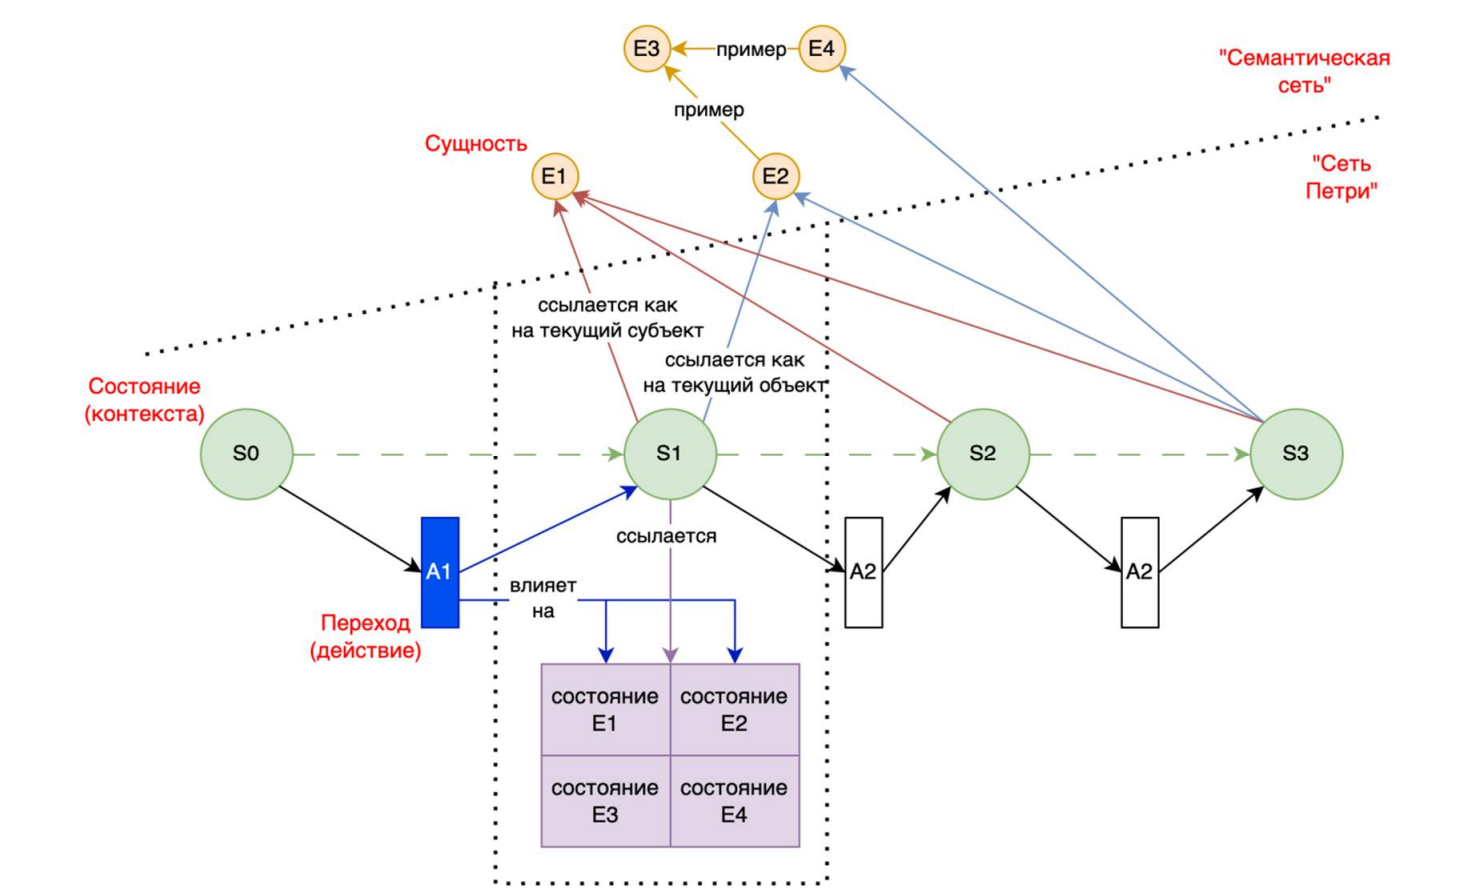
\includegraphics[width=0.6\linewidth]{inc/img/graph.png}
	\caption{Граф, описывающий инструкцию~\cite{graph}}
	\label{A1}
\end{figure}

\clearpage

\section{Пример экспертного разбора домена инструкций}

В качестве домена будет рассматриваться домен кухонных рецептов, так как они имеют чёткую структуру и легко доступны.

При выполнении инструкции система будет хранить текущий прогресс выполнения рецепта, определять следующий шаг выполнения и соответствующие рекомендации.
Для определения необходимых рекомендаций предлагается ввести систему меток для возможных действий в данном домене. 
Таким образом, задача системы сводится к отслеживанию прогресса, определению следующих действий, обработке хранимых меток, связанных с предложенным действием, и выдаче соответствующих меткам рекомендаций.

Для персонализации процесса поддержки пользователя для каждой подсказки СППР предлагается создать систему, позволяющую оператору выбрать свой уровень подготовки в кулинарии, позволяя давать различные рекомендации в зависимости от выбранного уровня.
Таким образом, если оператор новичок, он будет получать рекомендации отличные от тех, которые бы давались более опытным пользователям.
Система может, например, отдавать более высокий приоритет рекомендациям, связанным с безопасностью выполняемого действия.

Для повышения безопасности процесса также можно ввести метки, связанные с предупреждениями о необходимости повышенного внимания пользователя.
К таким действиям можно отнести, например, использование ножей и работу с кипятком.

Во многих рецептах есть необходимость выполнять действие в течение определённого времени.
Для отслеживания прогресса можно для таких действий ввести временную метку, при обработке которой СППР запустит таймер, напоминающий пользователю о завершении действия.

На практике во многих рецептах есть возможность заменить ингредиенты на некоторую альтернативу.
Для таких рецептов можно ввести метку замены, предлагающую пользователю при необходимости заменить ингредиенты в рецепте.
Поскольку такие замены индивидуальны для каждого блюда, такие разметки будет необходимо описывать для каждого рецепта отдельно, вместо их введения в качестве общей рекомендации. 

Таким образом, полученные в результате разбора предметной области метки и соответствующие им рекомендации сохраняются в базе знаний СППР. 
Поскольку существует возможность, что одновременно одно действие вызовет необходимость дать более одной рекомендации, для более качественной работы системы предлагается ввести алгоритм выбора порядка необходимых рекомендаций.
Простейшая реализация такого алгоритма заключается в присваивании каждому классу меток числового уровня приоритета и предоставлении рекомендаций согласно их важности.

Таким образом, каждое действие или состояние в домене будет представлено в базе знаний и будет иметь набор меток, описывающих необходимые рекомендации и их приоритетность.
Пример базы знаний СППР для рецептов представлен в таблице~\ref{tbl:marks}, соотношения меток и необходимых рекомендаций представлено в таблице~\ref{tbl:recomendations}.   

\begin{table}[h]
	\centering
	\begin{threeparttable}
		\caption{База знаний СППР для рецептов}
		\label{tbl:marks}
		
		\begin{tabularx}{\textwidth}{|X|X|X|}
			\hline
			\textbf{Класс}    & \textbf{Текст}                    & \textbf{Метки}                   \\
			\hline
			Действие  & Нарезать                 & Нож                     \\
			\hline
			Состояние & Кипячёное                & Кипяток                 \\
			\hline
			Действие  & Варить в течение 5 минут & Кипяток, таймер 5 минут \\
			\hline
		\end{tabularx}
	\end{threeparttable}
\end{table}

\begin{table}[h]
	\centering
	\begin{threeparttable}
		\caption{Пример соотношений меток и рекомендаций}
		\label{tbl:recomendations}
		
		\begin{tabularx}{\textwidth}{|X|X|X|}
			\hline
			\textbf{Приоритет}    & \textbf{Метка}                    & \textbf{Рекомендация}                   \\
			\hline
			1  & Нож                 & При нарезке защищайте пальцы                     \\
			\hline
			2 & Кипяток                & При работе с кипятком используйте перчатки                 \\
			\hline
			3 & Таймер 5 минут  & Напоминание: прошло 5 минут\\
			\hline
		\end{tabularx}
	\end{threeparttable}
\end{table}

\clearpage

\section{Планирование действий при ветвлении}
\subsection{Постановка проблемы}

Главной целью инструкции является достижение некоторой цели путём выполнения структурированной последовательности действий пользователем.
На практике в инструкциях часто вводят дополнительные шаги, которые направлены на решение ситуаций, возникающих в результате отклонения от оптимального пути достижения цели.
Например, если в результате готовки полученное блюдо получилось подгоревшим, рецепт может посоветовать пользователю убрать сгоревшие части, тем самым улучшая получившийся результат.

Таким образом, СППР, поддерживающая пользователя при выполнении инструкций и использующая граф в своей основе, должна обладать следующей функциональностью:
\begin{enumerate} 
    \item находить оптимальный путь движения по графу для достижения цели инструкции, заданной помеченной вершиной; 
    \item уметь корректно обрабатывать ветвления по ходу движения, предлагая пользователю корректные рекомендации при необходимости.
\end{enumerate}

Так как граф основан на инструкции, путь до конечного состояния инструкции из начального всегда будет существовать.
В случае отсутствия ветвления в инструкции, линейность инструкции означает возможность достижения конечной вершины графа путём движения по единственному возможному пути.

В случае возникновения ветвления, перед СППР возникнет необходимость выбрать один из нескольких вариантов пути.
Так как за исключением разметки экспертов у СППР нет иных данных для принятия решения, она будет использована в качестве основного источника информации о вариантах ветвления.

Следующие точки пути можно рассматривать как альтернативы, а метки экспертов как критерии оценки.
Для выбора из нескольких альтернатив подходят методы теории принятия решений.
Исследуем наиболее часто используемые методы, применяемые для сравнения альтернатив со слабоструктурированными критериями~\cite{comparison}.

\clearpage

\subsection{МАИ}

\textbf{Метод анализа иерархий} (МАИ) --- метод, представляющий проблему в виде иерархии целей, критериев и альтернатив~\cite{MAI}.
Метод был разработан Томасом Саати, после чего использовался по всему миру для решения проблем всех типов, начиная от управления государствами до решения частных проблем в бизнесе.
В его основе лежат парные сравнения и субъективные оценки предпочтений.

Метод анализа иерархий состоит из следующих шагов:
\begin{itemize} 
    \item построение качественной модели проблемы в виде иерархии, включающей цель, альтернативные варианты достижения цели и критерии для оценки качества альтернатив;
    \item определение приоритетов всех элементов иерархии;
    \item синтез глобальных приоритетов альтернатив;
    \item принятие решения на основе полученных результатов.
\end{itemize}

\subsection*{Моделирование проблемы в виде иерархии}

На первом этапе строится иерархическая структура, объединяющая цель выбора, критерии, альтернативы и другие факторы, влияющие на выбор решения.
Данный этап необходим для полноценного анализа проблемы.

\textbf{Иерархическая структура} является способом представления зависимости цели от выбранных критериев.
Иерархическая структура имеет не менее трёх уровней.
На верхнем уровне располагается цель, на нижнем находятся альтернативы, направленные на достижение цели, между ними --- критерии, их связывающие.
На рисунке~\ref{A4} приведён пример иерархической структуры МАИ.

\begin{figure}[H]
	\centering
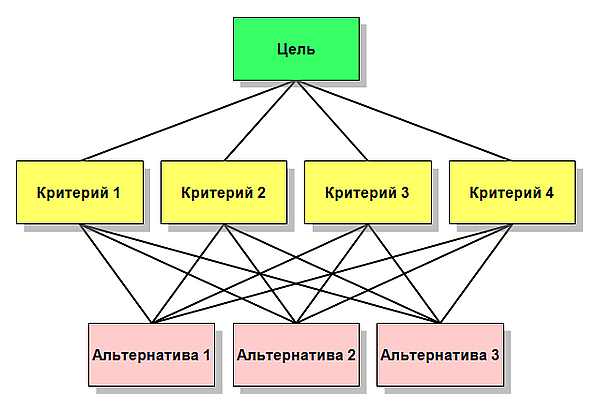
\includegraphics[width=0.6\linewidth]{inc/img/MAI.png}
	\caption{Иерархическая структура МАИ~\cite{MAI}}
	\label{A4}
\end{figure}

Отдельный элементом на каждом уровне называется \textbf{узлом}.
Элементы более высокого уровня, связанные с узлом, являются для него \textbf{родительскими}.
Для родительских элементов узел является \textbf{дочерним}.
Группы элементов с общим родительским элементов называются \textbf{группами сравнения}.
Родительские элементы альтернатив, как правило, исходящие из различных групп сравнения, называются покрывающими критериями.

Преимуществом такого представления является его гибкость --- иерархия будет меняться в зависимости от ЛПР.
В процессе выполнения МАИ иерархия также может меняться --- можно вносить критерии и альтернативы, если в процессе выполнения шагов МАИ они окажутся важными для ЛПР.

\subsection*{Расстановка приоритетов}

На следующем этапе ЛПР расставляет приоритеты для всех узлов структуры. 

\textbf{Приоритет} --- это число, представляющее собой относительный вес элемента в каждой группе.
Они могут принимать значения от нуля до единицы.
Большее значение означает большую значимость элемента с точки зрения ЛПР.
Сумма приоритетов элементов, подчинённых одному элементу выше лежащего уровня иерархии, равна единице.
Приоритет цели равен единице.

Приоритеты альтернатив относительно критериев называются \textbf{локальными}.
Для сравнения альтернатив, локальные приоритеты умножаются на приоритеты критериев и суммируются, полученное число является \textbf{глобальным} приоритетом альтернативы. 

На рисунке~\ref{A6} приведён пример иерархической структуры МАИ.

\begin{figure}[H]
	\centering
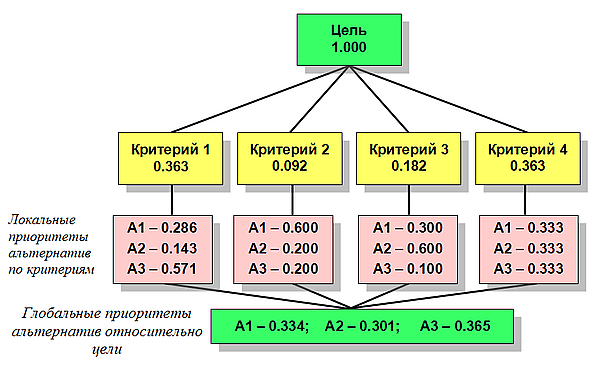
\includegraphics[width=0.6\linewidth]{inc/img/MAI_priority.png}
	\caption{Иерархическая структура МАИ с приоритетами~\cite{MAI}}
	\label{A6}
\end{figure}

В результате выбирается альтернатива с наибольшим значением глобального приоритета.

\subsection*{Нахождение локальных приоритетов}

В основе метода анализа иерархий лежит процедура парных сравнений элементов каждой группы сравнения.
Для количественной оценки предпочтений используется основная шкала Саати, приведённая в таблице~\ref{tab:saaty}.

\begin{table}[H]
	\centering
	\caption{Шкала относительной важности Саати}
	\label{tab:saaty}
	\begin{tabular}{|c|l|}
		\hline
		\textbf{Интенсивность важности} & \textbf{Определение} \\
		\hline
		1 & Одинаковая важность \\
		2 & Слабое превосходство \\
		3 & Умеренное превосходство \\
		4 & Существенное превосходство \\
		5 & Значительное превосходство \\
		6 & Очень сильное превосходство \\
		7 & Сильнейшее превосходство \\
		8 & Подавляющее превосходство \\
		9 & Абсолютное превосходство \\
		\hline
	\end{tabular}
\end{table}

Для каждой группы сравнения (критериев, подкритериев или альтернатив по отношению к родительскому элементу) заполняется матрица парных сравнений \(A = (a_{ij})\), где \(a_{ij}\) показывает превосходство элемента \(i\) над элементом \(j\). 
Матрица является обратно-симметричной, то есть \(a_{ij} = 1/a_{ji}\).
Диагональные элементы равны 1.

Пример заполненной матрицы попарных сравнений представлен на рисунке~\ref{fig:comparison_matrix}.
\begin{figure}[H]
	\centering
	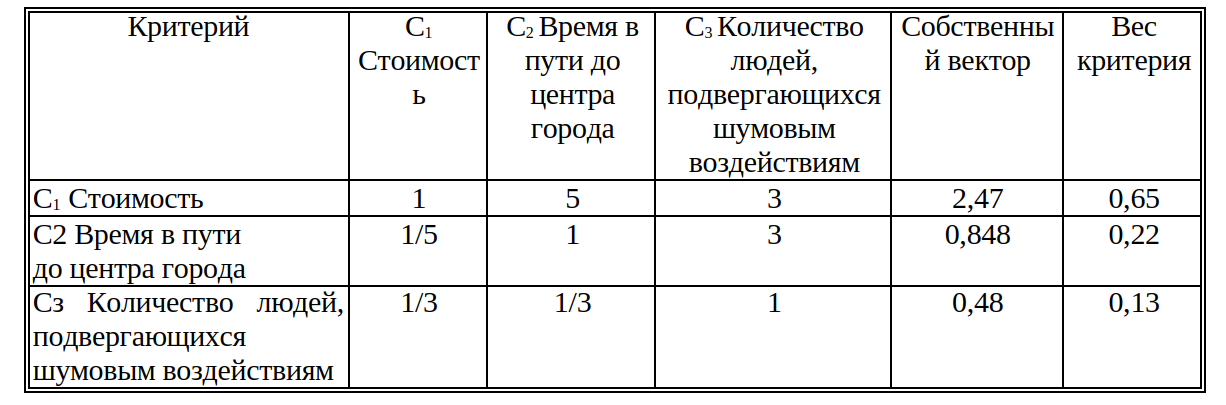
\includegraphics[width=0.8\linewidth]{inc/img/mai_comparison.png}
	\caption{Пример заполненной матрицы попарных сравнений~\cite{larichev}}
	\label{fig:comparison_matrix}
\end{figure}


\subsection*{Вычисление вектора приоритетов}

Для извлечения вектора приоритетов \(w = (w_1, w_2, \dots, w_n)\) из матрицы \(A\) применяется метод геометрического среднего (аппроксимация собственного вектора). 
Локальные приоритеты вычисляются по формуле:

\[
w_i = \frac{\left( \prod_{j=1}^{n} a_{ij} \right)^{1/n}}{ \sum_{k=1}^{n} \left( \prod_{j=1}^{n} a_{kj} \right)^{1/n} }, \quad i=1,\dots,n.
\]

Полученные веса нормированы: \(\sum_{i=1}^{n} w_i = 1\).

\subsection*{Проверка согласованности}

Для оценки качества экспертных суждений рассчитывается главное собственное значение \(\lambda_{\max}\) матрицы \(A\):

\[
\lambda_{\max} = \frac{1}{n} \sum_{i=1}^{n} \frac{(A w)_i}{w_i},
\]

где \((A w)_i = \sum_{j=1}^{n} a_{ij} w_j\) --- компонента произведения матрицы на вектор приоритетов.

Далее вычисляется индекс согласованности (ИС):

\[
\text{ИС} = \frac{\lambda_{\max} - n}{n-1}.
\]

Отношение согласованности (ОС) определяется как:

\[
\text{ОС} = \frac{\text{ИС}}{\text{СИ}},
\]

где СИ --- случайный индекс, соответствующий среднему значению ИС для случайных матриц того же порядка \(n\). Значения СИ для \(n\) от 1 до 10 приведены в таблице~\ref{tab:ri}.

\begin{table}[H]
\centering
\caption{Случайные индексы (СИ)}
\label{tab:ri}
\begin{tabular}{|c|c|c|c|c|c|c|c|c|c|c|}
\hline
\(n\) & 1 & 2 & 3 & 4 & 5 & 6 & 7 & 8 & 9 & 10 \\
\hline
СИ & 0.00 & 0.00 & 0.58 & 0.90 & 1.12 & 1.24 & 1.32 & 1.41 & 1.45 & 1.49 \\
\hline
\end{tabular}
\end{table}

Матрица считается согласованной, если \(\text{ОС} < 0.10\) (в отдельных задачах допускается \(\text{ОС} < 0.20\)).
При невыполнении этого условия эксперту рекомендуется пересмотреть значения в матрице попарных сравнений.

Данный подход позволяет перейти от парных сравнений, соответствующих более интуитивно понятным языковым определениям, к числовым приоритетам и оценить надежность полученных результатов.

\subsection*{Преимущества и недостатки}

К \textbf{преимуществам} метода можно отнести возможность явного учёта экспертных оценок и возможность учёта иерархической структуры.

К \textbf{недостаткам} можно отнести сложность масштабирования метода при росте количества критериев и альтернатив.


\clearpage

\subsection{ELECTRE}

\textbf{ELECTRE} --- это семейство алгоритмов, относящихся к многокритериальным методам принятия решений~\cite{ELECTRE}.
Впервые метод был предложен Бернандом Руа в 1968 году.
С тех пор было разработано множество его версий: ELECTRE I, ELECTRE II, ELECTRE III, ELECTRE IV, ELECTRE IS и ELECTRE TRI.

Отличительной особенностью методов этого семейства является поиск наилучшей альтернативы путём построения бинарных отношений между ними вместо использования весов.

Метод ELECTRE I состоит из следующих шагов:
\begin{itemize} 
    \item создание индексов;
    \item анализ большого количества альтернатив.
\end{itemize}

\subsection*{Шаг создания индексов}

К каждому критерию из общего множества критериев $N$ мощностью $n$ назначается в соответствие целое число $w$ --- вес критерия.
Вес критерия задаётся экспертами.

Далее выдвигается гипотеза о преимуществе альтернативы $A_i$ над $A_j$.
Для проверки гипотезы множество критериев $N$ разбивается на следующие подмножества: 
\begin{itemize} 
	\item $N^+$ --- подмножество критериев, по которым $A_i$ приоритетнее $A_j$; 
	\item $N^=$ --- подмножество критериев, по которым $A_i$ равноважна $A_j$; 
	\item $N^-$ --- подмножество критериев, по которым $A_j$ приоритетнее $A_u$.
\end{itemize}

На основе этих множеств рассчитывается индекс согласия $C_{{A_i}{A_j}}$:
\begin{equation}
	C_{{A_i}{A_j}} = \frac{\sum{_{n \in N^+ N^=} w_n}}{\sum{w_n}},
	\label{eq:electre_C}
\end{equation}
где:
\begin{itemize}
	\item $w_n$ --- заявленная экспертами важность (вес) $n$--го критерия;
	\item $A_i$, $A_j$ --- индексы, описывающие заявленную гипотезу о превосходстве $i$-й альтернативы над $j$-й;
	\item $n$ --- количество критериев.
\end{itemize}

Формула для расчёта индекса несогласия $d$ имеет вид:
\begin{equation}
	d_{{A_i}{A_j}} = {max}_{n \in N} \frac{l^n_{A_j} - l^n_{A_i}}{{L_n}},
	\label{eq:electre_d}
\end{equation}
где:
\begin{itemize}
	\item $l^n_{A_j}$, $l^n_{A_i}$ --- оценки альтернатив по $n$-му критерию;
	\item $A_i$, $A_j$ --- индексы, описывающие заявленную гипотезу о превосходстве $i$-й альтернативы над $j$-й;
	\item $L_n$ --- длина шкалы оценки $n$--го критерия;
	\item $n$ --- количество критериев.
\end{itemize}

Далее эксперты задают критические значения индекса согласия и несогласия.
Если индекс согласия выше соответствующего уровня или индекс несогласия ниже, то гипотеза считается верной и альтернатива считается превосходящей.
В ином случае, гипотеза считается неверной и альтернативы признаются несравнимыми.

\subsection*{Шаг изучения альтернатив}

Все альтернативы, не превосходящие остальные, исключаются из множества потенциальных наилучших альтернатив.
Оставшиеся альтернативы образуют множество, в котором все альтернативы либо несравнимы, либо равноважны.

Для уменьшения количества оставшихся альтернатив, эксперты уменьшают пороги уровней согласия и повышают пороги уровней несогласия.
Этот процесс продолжается до тех пор, пока в группе не останутся только наилучшие альтернативы.
Наилучшую альтернативу среди оставшихся можно выбрать с помощью некоторой целевой функции, подобранной специально под конкретную решаемую задачу.

\subsection*{Преимущества и недостатки}

К \textbf{преимуществам} метода можно отнести эффективность при слабой формализуемости, возможность использования конфликтных и неполных данных и отсутствие необходимости нормализации весов.

К \textbf{недостаткам} можно отнести необходимость настройки порогов и неоднозначность в результате ранжирования.

\clearpage

\subsection{TOPSIS}

\textbf{TOPSIS} (Technique for Order of Preference by Similarity to Ideal Solution) --- один из наиболее широко используемых методов многокритериального принятия решений~\cite{TOPSIS}.
Метод был разработан Хваном и Юном в 1981 году.

В основе метода лежит геометрическая интерпретация, лучшая альтернатива определяется как самая близкая к идеальному решению и самая дальняя от худшего решения.

Метод TOPSIS состоит из следующих шагов:
\begin{itemize} 
    \item построение матрицы решений;
    \item нормализация матрицы;
    \item построение взвешенной нормализованной матрицы;
    \item определение позитивного и негативного идеалов;
    \item нахождение расстояний до идеалов;
    \item нахождение относительной близости к идеалу.
\end{itemize}

\subsection*{Построение матрицы решений} 

Создаётся матрица $X = (x_{ij})$, где $(x_{ij})$ --- оценка $i$--ой альтернативы по $j$--му критерию.

\subsection*{Нормализация матрицы} 

Нормализуем матрицу по следующей формуле:
\begin{equation}
	r_{ij} = \frac{x_{ij}}{\sqrt{\sum_{i=1}^{m} x_{ij}^2}}.
	\label{eq:TOPSIS_rij}
\end{equation}

\subsection*{Построение взвешенной нормализованной матрицы} 

Каждому критерию экспертным путём назначается вес $w_j$, при этом $\sum{w_j} = 1$. 
Взвешенная нормализованная матрица $V = (v_{ij})$ рассчитывается путём умножения нормализованных оценок на веса:
\begin{equation}
	v_{ij} = w_j \cdot r_{ij}.
	\label{eq:TOPSIS_vij}
\end{equation}

\subsection*{Определение позитивного и негативного идеалов} 

Находим лучшие $v_j^+ = \max_i v_{ij}$ и худшие $v_j^- = \min_i v_{ij}$ значения по всем критериям.

\textbf{Позитивный идеал} $A^+ = \{ v_1^+, v_2^+, \dots, v_n^+ \}$ --- это гипотетическая альтернатива, которая имеет наилучшее значение по всем критериям,
а \textbf{негативный идеал} $A^- = \{ v_1^-, v_2^-, \dots, v_n^- \}$ --- наихудшие.

\subsection*{Нахождение расстояний до идеалов} 

Для каждой альтернативы вычисляется евклидово расстояние до обоих идеальных точек.

Расстояние до позитивного идеала $S_i^+$ рассчитывается по формуле:
\begin{equation}
	S_i^+ = \sqrt{\sum_{j=1}^n (v_{ij} - v_j^+)^2}.
	\label{eq:TOPSIS_SI-}
\end{equation}


Расстояние до негативного идеала $S_i^-$ рассчитывается по формуле:
\begin{equation}
	S_i^- = \sqrt{\sum_{j=1}^n (v_{ij} - v_j^-)^2}.
	\label{eq:TOPSIS_SI+}
\end{equation}

\subsection*{Нахождение относительной близости к идеалу} 

Итоговый коэффициент для каждой альтернативы вычисляется по формуле:
\begin{equation}
	C_i^* = \frac{S_i^-}{S_i^+ + S_i^-}
	\label{eq:TOPSIS_C}
\end{equation}

Коэффициент $C_i^*$ может принимать значения от 0 до 1.
Чем ближе он к 1, тем ближе альтернатива к позитивному идеалу и тем дальше от негативного идеала.

Таким образом, полученные коэффициенты ранжируются по убыванию и альтернатива с наибольшим значением считается наилучшей.

\subsection{Преимущества и недостатки}

К \textbf{преимуществам} метода можно отнести хорошую масштабируемость и высокую точность результата.

К \textbf{недостаткам} можно отнести зависимость от нормализации данных и отсутствие возможности работать с нечисловыми критериями.

\clearpage

\section{Сравнение методов планирования действий}
В качестве критериев для сравнения методов планирования действий были взяты следующие:
\begin{itemize}
	\item \textbf{K1} --- требование к числовым или категориальным данным;
	
	\item \textbf{K2} --- учёт субъективных факторов;
	
	\item \textbf{K3} --- поддержка неполных данных;
	
	\item  \textbf{К4} --- устойчивость к изменениям критериев и входных данных;
	
	\item  \textbf{К5} --- наличие ранжирования.
	
\end{itemize}

Результаты сравнительного анализа представлены в таблице~\ref{tbl:comparison}.
\begin{table}[h]
	\centering
	\begin{threeparttable}
		\caption{Сравнение подходов к планированию действий}
		\label{tbl:comparison}
		
		\begin{tabularx}{\textwidth}{|p{2.5cm}|p{3.5cm}|X|p{2cm}|p{2cm}|X|}
			\hline
			\textbf{Метод} & \textbf{К1} & \textbf{К2} & \textbf{К3} & \textbf{К4} & \textbf{К5} \\
			\hline
			МАИ & Категориальные & Да & Частично & Средняя & Да \\
			\hline
			ELECTRE & Смешанные & Да & Да & Высокая & Частично \\
			\hline
			TOPSIS & Числовые & Нет & Нет & Средняя & Да \\
			\hline
		\end{tabularx}
	\end{threeparttable}
\end{table}

В результате сравнения можно сделать вывод, что МАИ подходит в случае, если важны экспертные оценки и существует возможность создать иерархическую структуру.

Метод ELECTRE эффективен в конфликтных и слабо формализованных задачах, в том числе при отсутствии возможности использовать точные числовые оценки.

Метод TOPSIS подходит для задач с точными числовыми оценками, где необходима высокая точность результата.

Таким образом, для решения нашей задачи лучшим методом является МАИ, так как TOPSIS требует слишком высокого качества числовых данных, а ELECTRE требует дополнительного ранжирования после выполнения.